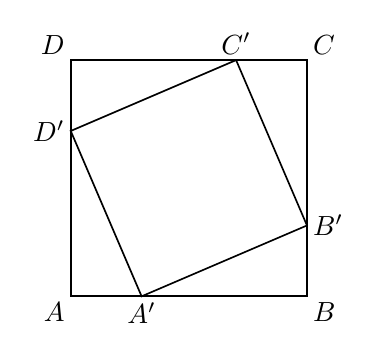
\begin{tikzpicture}[x=1cm,y=1cm,font=\normalsize,
 geometry edge/.style={solid,line width=.6pt},
 geometry mark/.style={solid,line width=.6pt},
 geometry label/.style={font=\normalsize,inner sep=2pt}]
\coordinate (A) at (0,0);
\coordinate (B) at (3,0);
\coordinate (C) at (3,3);
\coordinate (D) at (0,3);
\coordinate (Ap) at (0.9,0);
\coordinate (Bp) at (3,0.9);
\coordinate (Cp) at (2.1,3);
\coordinate (Dp) at (0,2.1);
\draw[geometry edge] (A)--(B)--(C)--(D)--cycle;
\draw[geometry edge] (Ap)--(Bp)--(Cp)--(Dp)--cycle;
\node[geometry label,below left] at (A) {$A$};
\node[geometry label,below right] at (B) {$B$};
\node[geometry label,above right] at (C) {$C$};
\node[geometry label,above left] at (D) {$D$};
\node[geometry label,below] at (Ap) {$A'$};
\node[geometry label,right] at (Bp) {$B'$};
\node[geometry label,above] at (Cp) {$C'$};
\node[geometry label,left] at (Dp) {$D'$};
\end{tikzpicture}
